%============================================================================
% tento soubor pouzijte jako zaklad
% (c) 2008 Michal Bidlo
% E-mail: bidlom AT fit vutbr cz
%============================================================================
% kodovanie: iso-8859-2 (zmena prikazem iconv, recode alebo cstocs)

\documentclass[cover]{projekt}
\usepackage[latin2]{inputenc}
\usepackage[T1, IL2]{fontenc}
\usepackage{url}
\DeclareUrlCommand\url{\def\UrlLeft{<}\def\UrlRight{>} \urlstyle{tt}}

\usepackage{array}
\usepackage{longtable}
\newcolumntype{M}[1]{>{\centering\arraybackslash}m{#1}}
\usepackage{makecell}
\renewcommand{\arraystretch}{1.45}

\ifx\pdfoutput\undefined % nejedeme pod pdflatexem
\else
  \usepackage{color}
  \usepackage[unicode,colorlinks,hyperindex,plainpages=false,pdftex]{hyperref}
  \definecolor{links}{rgb}{0.4,0.5,0}
  \definecolor{anchors}{rgb}{1,0,0}
  \def\AnchorColor{anchors}
  \def\LinkColor{links}
  \def\pdfBorderAttrs{/Border [0 0 0] }  % Bez okrajov okolo odkazov.
  \pdfcompresslevel=9
\fi

%Informacie o praci.
\projectinfo{
  project=OP,
  year=2015,
  title={Sledov�n� GSM a z�znamy ud�lost� oper�tory v �R},
  subject={Odborn� pr�ca do predmetu IBS},
  author={Luk� Vrabec}
}
\begin{document}
  	\maketitle
  	\tableofcontents
	%=========================== Uvod =================================
\chapter{Popis protokolu}

Bull's Authentication Protokol\cite{bull} bol predstaven� v roku 1997. Jeho autorom je J.Bull po ktorom nesie meno aj autentifika�n� protokol. �lohou tohto protokolu je distrib�cia 
nov�ch k���ov cez fixn� po�et klientov a server, pri�om ka�d� susedn� dvojica vlastn� jeden tak�to k���. 

Popis protokolu je nasledovn�. V prvom kroku �iadaj� ��astn�ci server o k���e pre dvojice susedn�ch klientov. T�to �iados� prebieha tak, �e klienti vytvoria ak�si "re�az", kedy prv� klient 
po�iada o k��� susedn�ho klienta, ten da��ieho susedn�ho klienta a� posledn� klient po�le zabalen� spr�vy so �iadostami o k���e serveru. Takto je vytvoren� "re�az" kedy s� spr�vy o �iados� 
k���a zabalen� rekurz�vne. V momente ked server pr�jme t�to zabalen� spr�vu, server vygeneruje rela�n� k���e pre dvojice klientov. Tieto dvojice k���ov s� odoslan� sp� najbli�siemu klientovi
(tomu, ktor� odosielal spr�vu serveru). N�sledne tento klient po�le spolo�n� k�u� pre dvojicu spolu so v�etk�mi zvy�n�mi k���ami sp� svojmu predchodzovi, tento �kon sa opakuje k�m nieje 
k��� odoslan� prv�mu klientovi. Grafick� reprezent�cia je obsiahnut� v obr�zku(1.1)

\begin{figure}[ht]
 \begin{center}
   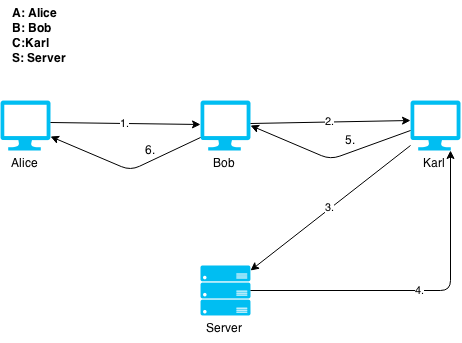
\includegraphics[scale=0.55]{fig/bull.png}
    \caption{Grafick� reprezent�cia protokolu}
 \end{center}
\end{figure}

\newpage

\noindent \texttt{A, B, C, S} :   	klienti a server \\
\texttt{Kab, Kbc} :   	symetrick� k�u�e pre dvojicu susedn�ch klientov \\
\texttt{Na, Nb, Nc} :   	��slo - nonce \\
\texttt{Kas, Kbs, Kcs} :   	 symetrick� k���e\\
\texttt{h }:   		hashovacia funkcia \\
\\
\noindent\texttt{A computes Xa = h((A,B,Na),Kas), (A,B,Na)} \\
\texttt{1.   	A 	-> 	B 	:   	Xa} \\
\texttt{B computes Xb = h((B,C,Nb,Xa),Kbs), (B,C,Nb,Xa)} \\
\texttt{2.   	B 	-> 	C 	:   	Xb} \\
\texttt{C computes Xc = h((C,S,Nc,Xb),Kcs), (C,S,Nc,Xb)} \\
\texttt{3.   	C 	-> 	S 	:   	Xc} \\
\texttt{4.   	S 	-> 	C 	:   	A, B, Kab xor h(Na,Kas), {A,B,Na}Kab,}\\
\texttt{  	  	  	  	  	B, A, Kab xor h(Nb,Kbs), {B,A,Nb}Kab,}\\
\texttt{  	  	  	  	  	B, C, Kbc xor h(Nb,Kbs), {B,C,Nb}Kbc,}\\
\texttt{  	  	  	  	  	C, B, Kbc xor h(Nc,Kcs), {C,B,Nc}Kbc}\\
\texttt{5.   	C 	-> 	B 	:   	A, B, Kab xor h(Na,Kas), {A,B,Na}Kab,}\\
\texttt{  	  	  	  	  	B, A, Kab xor h(Nb,Kbs), {B,A,Nb}Kab,}\\
\texttt{  	  	  	  	  	B, C, Kbc xor h(Nb,Kbs), {B,C,Nb}Kbc}\\
\texttt{6.   	B 	-> 	A 	:   	A, B, Kab xor h(Na,Kas), {A,B,Na}Kab}\\

\subsubsection{Zn�me �toky}
V roku 1998 bol publikovan� �tok na tento autentifika�n� protokol. �tok sa naz�va "domino attack". Tento �tok predstavili P. Y. A Ryan a S. A. Schneider\cite{utok}. K tomuto �toku je potrebn� aby �to�n�k bol v pomyselnej "re�azi" pri �iadan� a n�sledne
prij�man� susedn�ch k���ov. Ak je �to�n�k(Carl) posledn�m klientom, server mu (4. krok) po�le v�etky k���e pre dvojice klientov, teda zachyt� aj nasleduj�ce spr�vy: \texttt{Kab xor h(Nb,Kbs)} a \texttt{Kbc xor h(Nb,Kbs)}.
Carl pozn� k��� \texttt{Kbc}, a ked�e \texttt{Kab =  Kbc xor Kab xor h(Nb, Kbs) xor Kbc xor h(Nb,Kbs)}, takto Carl vlastn� k��� \texttt{Kab}, ktor� bol p�vodne ur�en� len pre Alice a Boba. 


\chapter{Analityck� anal�za chovania protokolu}

\begin{table}[h]
\scalebox{0.6}{
\begin{tabular}{|c|l|l|}
\hline
\multicolumn{1}{|l|}{Krok}                                                                    & Znalosti                                                                                                                                                                                                       & Predpoklady                                                                                                                                                                                                  \\ \hline
\multicolumn{1}{|l|}{\begin{tabular}[c]{@{}l@{}}Po�iato�n� \\ podminky\end{tabular}}          & \begin{tabular}[c]{@{}l@{}}A: A, B, S, Kas,Na\\ B: B,C,S, Kbs, Nb\\ C: C, S, Kcs, Nc\\ S: S, Kas, Kbs, Kcs\end{tabular}                                                                                        & \begin{tabular}[c]{@{}l@{}}A: S: Kas\\ B: S: Kbs\\ C: S: Kcs\\ S: A: Kas, S:B:Kbs, S:C: Kcs\end{tabular}                                                                                                     \\ \hline
\multicolumn{1}{|l|}{\begin{tabular}[c]{@{}l@{}}Cie�ov�\\ podmienky\end{tabular}}             & \begin{tabular}[c]{@{}l@{}}A: Kab\\ B: Kab, Kbc\\ C: Kbc\end{tabular}                                                                                                                                          & \begin{tabular}[c]{@{}l@{}}A: B: Kab\\ B: A: Kab, B: C: Kbc\\ C: B: Kbc\end{tabular}                                                                                                                         \\ \hline
\multicolumn{1}{|l|}{\begin{tabular}[c]{@{}l@{}}Zak�zan�\\ cie�ov� \\ podmienky\end{tabular}} & \begin{tabular}[c]{@{}l@{}}A: Kbs, Kcs, Kbc\\ B: Kas, Kcs\\ C: Kas, Kbs, Kab\end{tabular}                                                                                                                      &                                                                                                                                                                                                              \\ \hline
1                                                                                             & \begin{tabular}[c]{@{}l@{}}A: A, B, S, Kas, Na\\ B: B, C, S, Kbs, Na, Nb\\ C: C, S, Kcs, Nc\\ S: S, Kas, Kbs, Kcs\end{tabular}                                                                                 & \begin{tabular}[c]{@{}l@{}}A: B: A, Na, A: S: Kas\\ B: S: Kbs\\ C: S: Kcs\\ S: A: Kas, S: B: Kbs, S: C: Kcs\end{tabular}                                                                                     \\ \hline
2                                                                                             & \begin{tabular}[c]{@{}l@{}}A: A, B, S, Kas,Na\\ B: B, C, S, Kbs,Na, Nb\\ C: C, S, Kcs, A, Na, Nb, Nc\\ S: S, Kas, Kbs, Kcs\end{tabular}                                                                        & \begin{tabular}[c]{@{}l@{}}A: S: Kas, A: B: Na\\ B: S: Kbs, B: C: Na, Nb, A, B\\ C: S: Kcs, S: B: Kbs,\\ S: C: Kcs, S: A: Kas\end{tabular}                                                                   \\ \hline
3                                                                                             & \begin{tabular}[c]{@{}l@{}}A: A, B, S, Na, Kas\\ B: B, C, S, Kbs,Na, Nb\\ C: A, C, S, Kcs, Na, Nb, Nc\\ S: S, A, B, C, Kas, Kbs, Kcs, Na, Nb, Nc\end{tabular}                                                  & \begin{tabular}[c]{@{}l@{}}A: S: Kas, A: B: Na,\\ B: S: Kbs, B: C: Na, Nb, A, B\\ C: S: Kcs, A, B, C, Na, Nb, Nc\\ S: B: Kbs; S: C: Kcs; S: A: Kas\end{tabular}                                              \\ \hline
4                                                                                             & \begin{tabular}[c]{@{}l@{}}A: A, B, S, Kas,Na, \\ B: B, C, S, Kbs,Na, Nb\\ C: C, S, A, Kbc, Kcs, Na, Nb, m1, m2, m3, m4\\ S: S, A, B, C, Kas, Kbs, Kcs, Na, Nb, Nc\end{tabular}                                & \begin{tabular}[c]{@{}l@{}}A: S: Kas, A: B: Na,\\ B: S: Kbs, B: C: Na, Nb, A, B\\ C: S: Kcs, A, B, C, Na, Nb, Nc \\ S: B: Kbs, S: C: Kcs, m1, m2, m3, m4, S: A: Kas\end{tabular}                             \\ \hline
5                                                                                             & \begin{tabular}[c]{@{}l@{}}A: A, B, S, Kas, Na\\ B: B, C, S, Kab, Kbs, Kbc, Na, Nb, m1, m2, m3\\ C: C, A, S, Nc, Kcs, Kbc, Na, Nb, m1, m2, m3, m4\\ S: S, A, B, C, Kas, Kbs, Kcs, Na, Nb, Nc\end{tabular}      & \begin{tabular}[c]{@{}l@{}}A: S: Kas, A: B: Na,\\ B: S: Kbs, B: C: Na, Nb, A, B \\ C: S: Kcs, A, B, C, Na, Nb, Nc, C: B: m1, m2, m3,\\ S: B: Kbs, S: C: Kcs, m1, m2, m3, m4, S: A: Kas\end{tabular}          \\ \hline
6                                                                                             & \begin{tabular}[c]{@{}l@{}}A: A, B, S, Kas, Kab,Na, m1 \\ B: B, C, S, Kab, Kbs, Kbc,Na, Nb, m1, m2, m3\\ C: C, A, S, Kbc, Kcs, Na, Nb, m1, m2, m3, m4\\ S: S, A, B, C,  Kas, Kbs, Kcs, Na, Nb, Nc\end{tabular} & \begin{tabular}[c]{@{}l@{}}A: S: Kas, A: B: Na\\ B: S: Kbs, B: C: Na, Nb, A, B, B: A: m1 \\ C: S: Kcs, A, B, C, Na, Nb, Nc, C: B: m1, m2, m3,\\ S: B: Kbs, S: C: Kcs, m1, m2, m3, m4, S: A: Kas\end{tabular} \\ \hline
\end{tabular}}
\end{table}

\chapter{Anal�za komunik�cie BP z r�znych poh�adov subjektov}
Nasleduje anal�za komunik�cie jak je uveden� v �l�nku od Alvesa-fossa\cite{alves-foss}

\noindent \textbf{BP z poh�adu subjektu A:}


\begin{table}[h]
\begin{tabular}{|l|l|}
\hline
\textbf{Spr�va}                                     & \textbf{Popis}                       \\ \hline
\texttt{A1: A: computes Xa = h((A, B, Na), Kas), (A, B, Na)} & A vytvor� spr�vu                     \\ \hline
\texttt{A2: A->: Xa}                                          & A po�ele spr�vu                      \\ \hline
\texttt{A3: ->A: A, B, Kab xor h(Na, Kas), \{A, B, Na\}Kab}   & A pr�jme spr�vu		            \\ \hline
\texttt{A4: A: compute h(Na, Kas)}                           & A vypo��ta spr�vu                    \\ \hline
\texttt{A5: A: h(Na, Kas) xor (Kab xor h(Na, Kas))}          & A z�ska k���                         \\ \hline
\texttt{A6: A: decrypt \{A, B, Na\}Kab}                      & A de�ifruje spr�vu                   \\ \hline
\end{tabular}
\end{table}


\noindent \textbf{BP z poh�adu subjektu B:}
\noindent
\begin{table}[h]
\scalebox{0.9}{
\begin{tabular}{|l|l|}
\hline
\textbf{Spr�va}                                                                                                                                                                                                    & \textbf{Popis}                       \\ \hline
\texttt{B1: B: computes Xb = h((B, C, Nb, Xa), Kbs), (B, C, Nb, Xa)}                                                                                                                                                        & B vytvor� spr�vu                     \\ \hline
\texttt{B2: B->: Xb}                                                                                                                                                                                                         & B po�ele spr�vu                      \\ \hline
\texttt{\begin{tabular}[c]{@{}l@{}}B3: ->B: A, B, Kab xor h(Na, Kas), \{A, B, Na\}Kab,     \\ \hspace{10 mm} B, A, Kab xor h(Nb, Kbs), \{B, A, Nb\}Kab,\\ \hspace{10 mm} B, C, Kbc xor h(Nb, Kbs), \{B, C, Nb\}Kbc\end{tabular}} &\multicolumn{1}{c|}{B pr�jme spr�vu} \\ \hline
\texttt{B4: B: compute h(Nb, Kbs)}                                                                                                                                                                                          & B vypo��ta spr�vu                    \\ \hline
\texttt{B5: B: h(Nb, Kbs) xor (Kab xor h(Nb, Kbs))}                                                                                                                                                                         & B z�ska k��� Kab                     \\ \hline
\texttt{B6: B: decrypt \{B, A, Nb\}Kab}                                                                                                                                                                                     & B de�ifruje spr�vu                   \\ \hline
\texttt{B7: B: h(Nb, Kbs) xor (Kbc xor h(Nb, Kbs))}                                                                                                                                                                         & B z�ska k��� Kbc                     \\ \hline
\texttt{B8: B: decrypt \{B, C, Nb\}Kbc}                                                                                                                                                                                     & B de�ifruje spr�vu                   \\ \hline
\texttt{B9: B->: A, B, Kab xor h(Na, Kas), \{A, B, Na\}Kab}                                                                                                                                                                  & B po�le spr�vu                       \\ \hline
\end{tabular}}
\end{table}

\noindent \textbf{BP z poh�adu subjektu C:}
\begin{table}[h]
\scalebox{0.8}{
\begin{tabular}{|l|l|}
\hline
\textbf{Spr�va}                                                                                                                                                                                                                  & \textbf{Popis}                       \\ \hline
\texttt{C1: C: computes Xc = h((C, S, Nc, Xb), Kcs), (C, S, Nc, Xb)}                                                                                                                                                                     & C vytvor� spr�vu                     \\ \hline
\texttt{C2: C->: Xc}                                                                                                                                                                                                                       & C po�ele spr�vu                      \\ \hline
\texttt{\begin{tabular}[c]{@{}l@{}}C3: ->C: A, B, Kab xor h(Na, Kas), \{A, B, Na\}Kab,\\ \hspace{10 mm} B, A, Kab xor h(Nb, Kbs), \{B, A, Nb\}Kab,\\ \hspace{10 mm} B, C, Kbc xor h(Nb, Kbs), \{B, C, Nb\}Kbc,\\ \hspace{10 mm} C, B, Kbc xor h(Nc, Kcs), \{C, B, Nc\}Kbc\end{tabular}} & \multicolumn{1}{c|}{C pr�jme spr�vu} \\ \hline
\texttt{C4: C: compute h(NC, Kcs)}                                                                                                                                                                                                        & C vypo��ta spr�vu                    \\ \hline
\texttt{C5: C: h(Nc, Kcs) xor (Kbc xor h(Nc, Kcs))}                                                                                                                                                                                       & C z�ska k��� Kab                     \\ \hline
\texttt{C6: C: decrypt \{B,C, Nc\}Kbc}                                                                                                                                                                                                    & C de�ifruje spr�vu                   \\ \hline
\texttt{\begin{tabular}[c]{@{}l@{}}C7: C->: A, B, Kab xor h(Na, Kas), \{A, B, Na\}Kab,\\  \hspace{10 mm} B, A, Kab xor h(Nb, Kbs), \{B, A, Nb\}Kab,\\  \hspace{10 mm} B, C, Kbc xor h(Nb, Kbs), \{B, C, Nb\}Kbc\end{tabular}}                                            & C po�le spr�vy                       \\ \hline
\end{tabular}}
\end{table}

\noindent \textbf{BP z poh�adu subjektu S:}

\begin{table}[h]
\scalebox{0.8}{
\begin{tabular}{|l|l|}
\hline
\textbf{Spr�va}                                                                                                                                                                                                                          & \textbf{Popis}                        \\ \hline
\texttt{S3: ->S: Xc}                                                                                                                                                                                                                               & S pr�jme spr�vu                       \\ \hline
\texttt{\begin{tabular}[c]{@{}l@{}}S1: S: compute: A, B, Kab xor h(Na, Kas), \{A, B, Na\}Kab,\\ \hspace{10 mm} B, A, Kab xor h(Nb, Kbs), \{B, A, Nb\}Kab,\\ \hspace{10 mm} B, C, Kbc xor h(Nb, Kbs), \{B, C, Nb\}Kbc,\\\hspace{10 mm} C, B, Kbc xor h(Nc, Kcs), \{C, B, Nc\}Kbc\end{tabular}} & \multicolumn{1}{c|}{S vytvor� spr�vu} \\ \hline                                                                                                                                                                                                        & S de�ifruje spr�vu                    \\ \hline
\texttt{\begin{tabular}[c]{@{}l@{}}S2: S->: A, B, Kab xor h(Na, Kas), \{A, B, Na\}Kab,\\ \hspace{10 mm} B, A, Kab xor h(Nb, Kbs), \{B, A, Nb\}Kab,\\ \hspace{10 mm} B, C, Kbc xor h(Nb, Kbs), \{B, C, Nb\}Kbc,\\\hspace{10 mm} C, B, Kbc xor h(Nc, Kcs), \{C, B, Nc\}Kbc\end{tabular}}         & S po�le spr�vy                        \\ \hline
\end{tabular}}
\end{table}

\chapter{Anal�za chovania protkolu pomocou automatick�ho n�stroja}
Pri pou�it� n�stroja \textbf{SPAN} boli pou�it� 3 z 4 met�d. Met�dy OFMC, ATSE, TA4SP vyhodnotili zdrojov� k�d protokolu ako bezpe�n�. Bohu�ia� grafick� reprezent�cia t�chto met�d nebola spr�vne ukon�en�, tak�e
je mo�n� �e pri p�san� k�du protokolu pri�lo k chybe. Met�du SATMC sa mi nepodarilo spusti�, nako�ko n�stroj SPAN nevygeneroval �iadne v�sledky.
 % obsah.tex
	\ifslovak
	  	\bibliographystyle{czechiso}
	\else 
  		\bibliographystyle{plain}
	\fi
  	\begin{flushleft}
 		\bibliography{literatura} % literatura.bib
  	\end{flushleft}

\end{document}
